% Página
\section{Recuperando Custódia das Chaves}

Em um cenário em que Bob perde sua Chave Mestra (MKBob.hex), ele solicita à custodiante Alice que criptografe suas duas chaves, Chave Privada (KPrBob.pem) e Chave de Dados (DEKBob.bin), com a Nova Chave Mestra (NMKBob.hex).

\subsection{Gerando Nova Chave Mestra - Bob}

\begin{figure}[H]
	\centering
	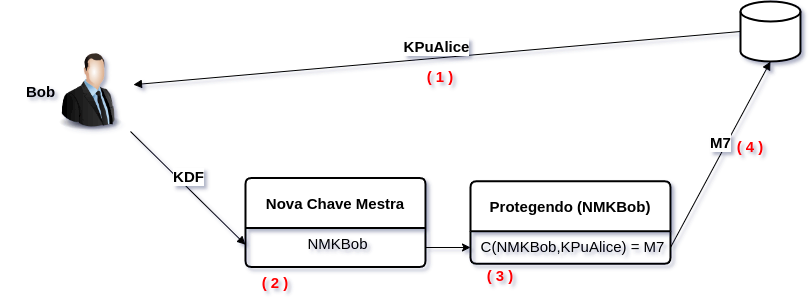
\includegraphics[scale=0.55]{nova-custodia_01.png}
	\caption{Processos de criação da Nova Chave Mestra do Bob}
	\label{fig:nova-custodia_01}
\end{figure}

\begin{enumerate}
	\item Bob recupera a Chave Pública da Alice (KPuAlice.pem) que está armazenada no servidor;
	\item Utilizando uma Key Derivation Function (KDF), Bob gera uma Nova Chave Mestra (NMKBob.hex);
	\begin{tcolorbox}[width=\textwidth]
		{\scriptsize
			\begin{verbatim}
				$ read -rs MASTER_PASSWORD
				$ SALT_HEX=$(openssl rand -hex 16)
				$ printf '%s' "$SALT_HEX" > NMKBob.salt
				$ openssl kdf -keylen 32 -kdfopt digest:SHA256 \
				  -kdfopt pass:"$MASTER_PASSWORD" -kdfopt salt:"$SALT_HEX" \
				  -kdfopt iter:600000 PBKDF2 | tr -d ':\n' > NMKBob.hex
			\end{verbatim}
		}
	\end{tcolorbox}
	\item Utilizando a Chave Pública da Alice (KPuAlice.pem), Bob protege sua Nova Chave Mestra (NMKBob.hex), gerando o Texto Cifrado M7;
	\begin{tcolorbox}[width=\textwidth]
		{\scriptsize
			\begin{verbatim}
			$ openssl pkeyutl -encrypt -inkey KPuAlice.pem -pubin -in NMKBob.hex -out M7.bin \
			  -pkeyopt rsa_padding_mode:oaep -pkeyopt rsa_oaep_md:sha256
			\end{verbatim}
		}
	\end{tcolorbox}
	\item O Texto Cifrado M7 é enviado para o servidor.
\end{enumerate}

\subsection{Nova Custódia - Alice}

\begin{figure}[H]
	\centering
	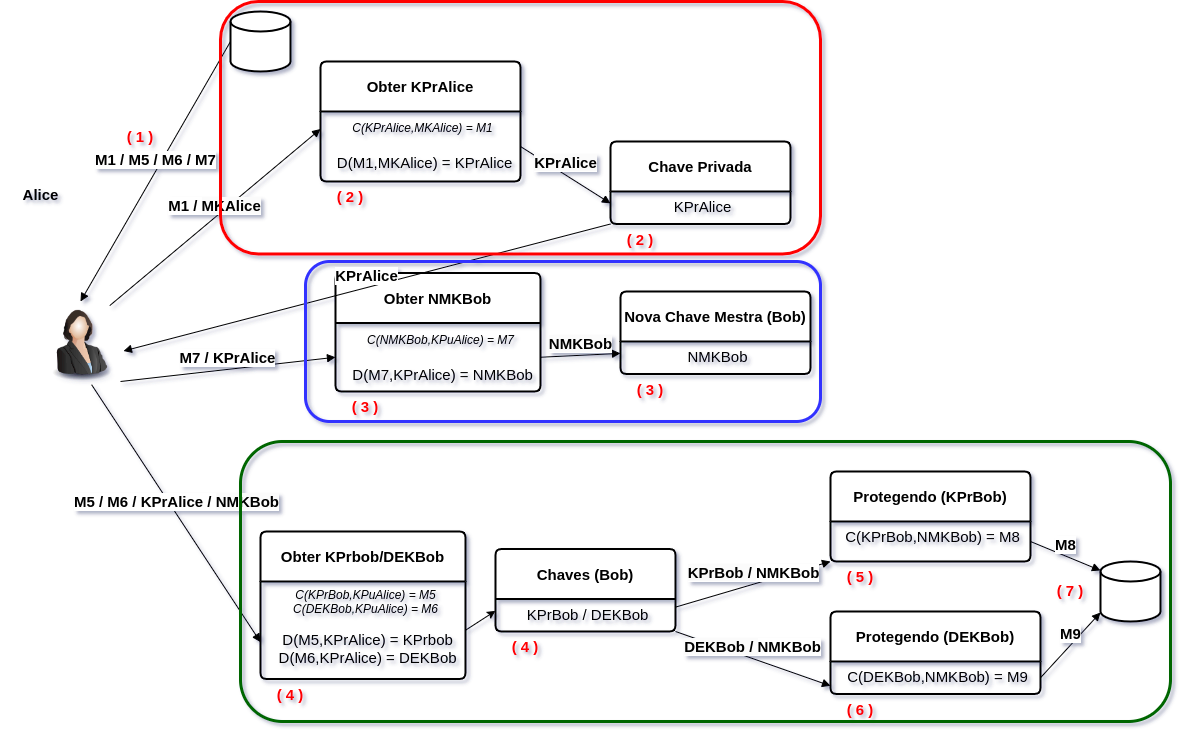
\includegraphics[scale=0.45]{nova-custodia_02.png}
	\caption{Processos de proteção das chaves do Bob com a sua Nova Chave Mestra}
	\label{fig:nova-custodia_02}
\end{figure}

\begin{enumerate}
	\item Alice faz o download dos Textos Cifrados M1, M5, M6 e M7 do servidor;
	\item Alice descriptografa o Texto Cifrado M1 com sua Chave Mestra (MKAlice.hex) e o IV associado para obter sua Chave Privada (KPrAlice.pem);
	\begin{tcolorbox}[width=\textwidth]
		{\scriptsize
			\begin{verbatim}
			$ openssl enc -d -aes-256-cbc -K "$(cat MKAlice.hex)" -iv "$(cat M1.iv)" \
			  -in M1.bin -out KPrAlice.pem
			\end{verbatim}
		}
	\end{tcolorbox}
	\item Com sua Chave Privada (KPrAlice.pem), Alice descriptografa o Texto Cifrado M7 e obtém a Nova Chave Mestra (NMKBob.hex) do Bob;
	\begin{tcolorbox}[width=\textwidth]
		{\scriptsize
			\begin{verbatim}
			$ openssl pkeyutl -decrypt -inkey KPrAlice.pem -in M7.bin -out NMKBob.hex \
			  -pkeyopt rsa_padding_mode:oaep -pkeyopt rsa_oaep_md:sha256
			\end{verbatim}
		}
	\end{tcolorbox}
	\item Com sua Chave Privada (KPrAlice.pem), Alice recupera os artefatos de custódia M5 e M6 e obtém a Chave Privada do Bob (KPrBob.pem) e a Chave de Dados do Bob (DEKBob.bin);
	\begin{tcolorbox}[width=\textwidth]
		{\scriptsize
			\begin{verbatim}
			$ openssl cms -decrypt -in M5.pem -inform PEM -recip Alice.cert.pem \
			  -inkey KPrAlice.pem -out KPrBob.pem

			$ openssl pkeyutl -decrypt -inkey KPrAlice.pem -in M6.bin -out DEKBob.bin \
			  -pkeyopt rsa_padding_mode:oaep -pkeyopt rsa_oaep_md:sha256
			\end{verbatim}
		}
	\end{tcolorbox}
	\item Com a Nova Chave Mestra do Bob (NMKBob.hex), Alice criptografa a Chave Privada do Bob (KPrBob.pem) gerando o Texto Cifrado M8;
	\begin{tcolorbox}[width=\textwidth]
		{\scriptsize
			\begin{verbatim}
			$ IV_HEX=$(openssl rand -hex 16)
			$ printf '%s' "$IV_HEX" > M8.iv
			$ openssl enc -aes-256-cbc -K "$(cat NMKBob.hex)" -iv "$IV_HEX" \
			  -in KPrBob.pem -out M8.bin
			\end{verbatim}
		}
	\end{tcolorbox}
	\item Com a Nova Chave Mestra do Bob (NMKBob.hex), Alice criptografa a Chave de Dados do Bob (DEKBob.bin) gerando o Texto Cifrado M9;
	\begin{tcolorbox}[width=\textwidth]
		{\scriptsize
			\begin{verbatim}
			$ IV_HEX=$(openssl rand -hex 16)
			$ printf '%s' "$IV_HEX" > M9.iv
			$ openssl enc -aes-256-cbc -K "$(cat NMKBob.hex)" -iv "$IV_HEX" \
			  -in DEKBob.bin -out M9.bin
			\end{verbatim}
		}
	\end{tcolorbox}
	\item Os Textos Cifrados M8 e M9 são enviados para o servidor.
\end{enumerate}

A partir deste ponto, a Chave Privada do Bob (KPrBob.pem) e a Chave de Dados do Bob (DEKBob.bin) estão protegidas com a Nova Chave Mestra do Bob (NMKBob.hex) e estão armazenadas no servidor. Os IVs M8.iv e M9.iv acompanham os respectivos textos cifrados.

\pagebreak

%Copyright
\vspace*{\fill}
\begin{flushright}
	\underline{\textit{Copyright}}\\
	All rights reserved to MT4 Tecnologia LTDA.\bigskip

	\underline{\textit{Autor}}\\
	Caio Abreu Ferreira [\href{mailto:cferreira@senhasegura.com}{cferreiras@senhasegura.com}] \bigskip\\
	
	\underline{\textit{MT4 Tecnologia Ltda.}}\\
	Rua Joaquim Antunes, 767 – Pinheiros – São Paulo\\
	Phone: +55 11 3065-7070\\
	\url{www.mt4.com.br}\\
\end{flushright}
